\section{Ćwiczenia 8: 27-IV-2017}
Przez $p_{ij}(t)$ we wszystkich zadaniach oznaczamy prawdopodobieństwo przejścia ze stanu $i$ do stanu $j$ w $t$ krokach.

\subsection{Zadania domowe A}
\paragraph{A1} Żaba siedzi nad strumieniem i co minutę,
z prawdopodobieństwem $p = \frac{1}{3}$ skacze na drugi brzeg, a z prawdopodobieństwem $q = \frac{2}{3}$ nie rusza się z miejsca. Niech $X_n$ będzie położeniem żaby (numerem brzegu strumienia) po $n$ minutach. $(X_n)$ jest zatem łańcuchem Markowa na zbiorze stanów $S = \{1, 2\}$.
\begin{enumerate}[label=\alph*)]
\item Przedstaw ten łańcuch za pomocą grafu skierowanego, którego wierzchołkami są oba stany, a strzałkom (w tym pętlom) przyporządkowane są odpowiednie prawdopodobieństwa przejścia ze stanu do stanu.

\begin{figure}[H]
\centering
\begin{tikzpicture}[shorten >=1pt, auto, node distance=3cm, ultra thick,main node/.style={circle,draw,minimum size=.4cm,inner sep=0pt}]
\begin{scope}[every node/.style={font=\sffamily\large\bfseries}]
\node [main node](v1) at (0,0) {1};
\node [main node](v2) at (2,0) {2};
\end{scope}
\path 
	(v1) edge [->,bend left] node {$\sfrac{1}{3}$} (v2)
    	 edge [loop above]   node {$\sfrac{2}{3}$} (v1)
    (v2) edge [->,bend left] node {$\sfrac{1}{3}$} (v1)
    	 edge [loop above]   node {$\sfrac{2}{3}$} (v2)
         ;
\end{tikzpicture}
\end{figure}
\item Wyznacz macierz przejścia $\mathbb{P}$ dla tego łańcucha.
$$\mathbb{P}=\begin{bmatrix}
\sfrac{2}{3}&\sfrac{1}{3}\\
\sfrac{1}{3}&\sfrac{2}{3}
\end{bmatrix}$$
\item Załóżmy, że na początku żaba jest na brzegu nr 1. Jakie jest prawdopodobieństwo, że po 3 minutach znajdzie się na drugim brzegu? Proszę obliczyć to prawdopodobieństwo bez podnoszenia do potęgi macierzy $\mathbb{P}$.

\textbf{Odpowiedź:} Możliwe ścieżki żaby:
$1\rightarrow 1\rightarrow 1\rightarrow 2$,
$1\rightarrow 1\rightarrow 2\rightarrow 2$,
$1\rightarrow 2\rightarrow 1\rightarrow 2$,
$1\rightarrow 2\rightarrow 2\rightarrow 2$
\begin{align*}
&\frac{2}{3}*\frac{2}{3}*\frac{1}{3}+\frac{2}{3}*\frac{1}{3}*\frac{2}{3}+\frac{1}{3}*\frac{1}{3}*\frac{1}{3}+\frac{1}{3}*\frac{2}{3}*\frac{2}{3}=\\
&\frac{4}{27}+\frac{4}{27}+\frac{1}{27}+\frac{4}{27} = \frac{13}{27}
\end{align*}
\item Oblicz $\mathbb{P}^3$ i odczytaj z niej $p_{12}(3)$. Czy wynik jest taki sam, jak w poprzednim podpunkcie?
\begin{align*}
&\mathbb{P}=\begin{bmatrix}
\sfrac{2}{3}&\sfrac{1}{3}\\
\sfrac{1}{3}&\sfrac{2}{3}
\end{bmatrix}\\
&\mathbb{P}^3=\begin{bmatrix}
\sfrac{2}{3}&\sfrac{1}{3}\\
\sfrac{1}{3}&\sfrac{2}{3}
\end{bmatrix}\begin{bmatrix}
\sfrac{2}{3}&\sfrac{1}{3}\\
\sfrac{1}{3}&\sfrac{2}{3}
\end{bmatrix}\begin{bmatrix}
\sfrac{2}{3}&\sfrac{1}{3}\\
\sfrac{1}{3}&\sfrac{2}{3}
\end{bmatrix}=\begin{bmatrix}
\sfrac{14}{27}&\sfrac{13}{27}\\
\sfrac{13}{27}&\sfrac{14}{27}
\end{bmatrix}
\end{align*}
\item Załóżmy, że na początku żaba jest na brzegu nr 1. Wyznacz $\bar{p}(1), \bar{p}(2)$ i $\bar{p}(3)$, czyli rozkłady prawdopodobieństwa dla położenia żaby po 1, 2, 3 minutach.

\begin{multicols}{2}
\begin{align*}
&\mathbb{P}=\begin{bmatrix}
\sfrac{2}{3}&\sfrac{1}{3}\\
\sfrac{1}{3}&\sfrac{2}{3}
\end{bmatrix}\\
&\mathbb{P}^2=\begin{bmatrix}
\sfrac{5}{9}&\sfrac{4}{9}\\
\sfrac{4}{9}&\sfrac{5}{9}
\end{bmatrix}\\
&\mathbb{P}^3=\begin{bmatrix}
\sfrac{14}{27}&\sfrac{13}{27}\\
\sfrac{13}{27}&\sfrac{14}{27}
\end{bmatrix}\\
&\bar{p}(1)=\begin{bmatrix}
\sfrac{2}{3}&\sfrac{1}{3}
\end{bmatrix}\\
&\bar{p}(2)=\begin{bmatrix}
\sfrac{5}{9}&\sfrac{4}{9}
\end{bmatrix}\\
&\bar{p}(3)=\begin{bmatrix}
\sfrac{14}{27}&\sfrac{13}{27}
\end{bmatrix}
\end{align*}
\end{multicols}
\item Załóżmy, że rozkład początkowy żaby to $\bar{p}(0) = \left[ \frac{1}{2}, \frac{1}{2}\right]$, tzn. z jednakowym prawdopodobieństwem znajduje się na brzegu 1 i na brzegu 2. Jakie jest prawdopodobieństwo, że po 3 minutach znajdzie się na brzegu 1?

\textbf{Odpowiedź: }
$$\frac{1}{2}*\frac{14}{27}+\frac{1}{2}*\frac{13}{27}=\frac{1}{2}$$
\end{enumerate}

\paragraph{A2} Obok podana jest macierz przejścia pewnego łańcucha Markowa o zbiorze stanów $S = \{1, 2, 3, 4, 5\}$.
$$\mathbb{P}=\begin{bmatrix}
\frac{1}{5}&\frac{1}{5}&\frac{1}{5}&\frac{1}{5}&\frac{1}{5}&\\
0&\frac{1}{2}&0&\frac{1}{2}&0\\
\frac{2}{3}&0&\frac{1}{6}&0&\frac{1}{6}&\\
0&0&0&1&0\\
\frac{1}{4}&0&\frac{1}{4}&0&\frac{1}{2}&
\end{bmatrix}$$
\begin{enumerate}[label=\alph*)]
\item Znajdź $p_{13}(2)$.

$$\mathbb{P}^2= \frac{1}{1800}\begin{bmatrix}
402 & 252 & 222 & 612 & 312\\
0 & 450 & 0 & 1350 & 0\\
515 & 240 & 365 & 240 & 440\\
0 & 0 & 0 & 1800 & 0\\
615 & 90 & 390 & 90 & 615
\end{bmatrix}$$
$p_{13}(2)=\sfrac{222}{1800}=\sfrac{37}{300}$
\item Znajdź $p_{23}(100)$.

$p_{23}(100) = 0$
\begin{figure}[H]
\centering
\begin{tikzpicture}[shorten >=1pt, auto, node distance=3cm, ultra thick,main node/.style={circle,draw,minimum size=.4cm,inner sep=0pt}]
\begin{scope}[every node/.style={font=\sffamily\large\bfseries}]
\node [main node](v1) at (-1,0) {1};
\node [main node](v2) at (-1,2) {2};
\node [main node](v3) at (2,3) {3};
\node [main node](v4) at (1,-1) {4};
\node [main node](v5) at (4,-2) {5};
\end{scope}
\path 
	(v1) edge [loop left] node {$\sfrac{1}{5}$} (v1)
    	 edge [->,bend left] node {$\sfrac{1}{5}$} (v2)
    	 edge [->] node {$\sfrac{1}{5}$} (v3)
         edge [->,bend left] node {$\sfrac{1}{5}$} (v4)
         edge [->,bend left] node {$\sfrac{1}{5}$} (v5)
    (v2) edge [->,bend left] node {$\sfrac{1}{2}$} (v4)
    	 edge [loop above]   node {$\sfrac{1}{2}$} (v2)
    (v3) edge [->,bend left] node {$\sfrac{2}{3}$} (v1)
    	 edge [loop above] node {$\sfrac{1}{6}$} (v3)
         edge [->,bend left] node {$\sfrac{1}{6}$} (v5)
    (v4) edge [loop right] node {$1$} (v4)     
    (v5) edge [->,bend left] node {$\sfrac{1}{4}$} (v1)
    	 edge [->] node {$\sfrac{1}{4}$} (v3)
         edge [loop below] node {$\sfrac{1}{2}$} (v5)
         ;
\end{tikzpicture}
\caption*{Napisane, że w grafie jest zero nic nie daje...\\Jak widać, z wierzchołka 2 można przejść do niego samego albo do wierzchołka 4, z którego można przejść Tylko do niego samego, więc z wierzchołka 2 do wierzchołka 3 nie da się ,,przejść''.}
\end{figure}
\item Wyznacz rozkład prawdopodobieństwa dla tego łańcucha po pierwszym kroku, przy założeniu, że rozkładem początkowym łańcucha jest $\bar{p}(0) = \left[ \frac{1}{2} , \frac{1}{3} , 0, 0, \frac{1}{6} \right]$.

\begin{align*}
\bar{p}(t) &= \bar{p}(0) * \mathbb{P}^t\\
\bar{p}(t) &= \bar{p}(t-1)*\mathbb{P}\\
\bar{p}(1) &= \left[ \frac{1}{2} , \frac{1}{3} , 0, 0, \frac{1}{6} \right] * \begin{bmatrix}
\frac{1}{5}&\frac{1}{5}&\frac{1}{5}&\frac{1}{5}&\frac{1}{5}&\\
0&\frac{1}{2}&0&\frac{1}{2}&0\\
\frac{2}{3}&0&\frac{1}{6}&0&\frac{1}{6}&\\
0&0&0&1&0\\
\frac{1}{4}&0&\frac{1}{4}&0&\frac{1}{2}&
\end{bmatrix} = \left[ \frac{17}{120}, \frac{4}{15}, \frac{17}{120}, \frac{4}{15}, \frac{11}{60}\right]
\end{align*}
\item Przedstaw rozważany łańcuch Markowa za pomocą grafu skierowanego o 5 wierzchołkach.
\begin{figure}[H]
\centering
\begin{tikzpicture}[shorten >=1pt, auto, node distance=3cm, ultra thick,main node/.style={circle,draw,minimum size=.4cm,inner sep=0pt}]
\begin{scope}[every node/.style={font=\sffamily\large\bfseries}]
\node [main node](v1) at (-1,0) {1};
\node [main node](v2) at (-1,2) {2};
\node [main node](v3) at (2,3) {3};
\node [main node](v4) at (1,-1) {4};
\node [main node](v5) at (4,-2) {5};
\end{scope}
\path 
	(v1) edge [loop left] node {$\sfrac{1}{5}$} (v1)
    	 edge [->,bend left] node {$\sfrac{1}{5}$} (v2)
    	 edge [->] node {$\sfrac{1}{5}$} (v3)
         edge [->,bend left] node {$\sfrac{1}{5}$} (v4)
         edge [->,bend left] node {$\sfrac{1}{5}$} (v5)
    (v2) edge [->,bend left] node {$\sfrac{1}{2}$} (v4)
    	 edge [loop above]   node {$\sfrac{1}{2}$} (v2)
    (v3) edge [->,bend left] node {$\sfrac{2}{3}$} (v1)
    	 edge [loop above] node {$\sfrac{1}{6}$} (v3)
         edge [->,bend left] node {$\sfrac{1}{6}$} (v5)
    (v4) edge [loop right] node {$1$} (v4)     
    (v5) edge [->,bend left] node {$\sfrac{1}{4}$} (v1)
    	 edge [->] node {$\sfrac{1}{4}$} (v3)
         edge [loop below] node {$\sfrac{1}{2}$} (v5)
         ;
\end{tikzpicture}
\end{figure}
\end{enumerate}


\paragraph{A3} Znajdź $p_{54}(5)$, jeżeli macierz przejścia łańcucha Markowa o zbiorze stanów $S = \{1, 2, 3, 4, 5\}$ jest:
$$\mathbb{P}=\begin{bmatrix}
0&0&0&\frac{1}{4}&\frac{3}{4}\\
0&0&0&\frac{1}{2}&\frac{1}{2}\\
0&0&\frac{2}{3}&0&\frac{1}{3}\\
\frac{1}{4}&\frac{3}{4}&0&0&0\\
\frac{3}{5}&\frac{2}{5}&0&0&0
\end{bmatrix}$$

\begin{figure}[H]
\centering
\begin{tikzpicture}[shorten >=1pt, auto, node distance=3cm, ultra thick,main node/.style={circle,draw,minimum size=.4cm,inner sep=0pt}]
\begin{scope}[every node/.style={font=\sffamily\large\bfseries}]
\node [main node](v1) at (5,2) {1};
\node [main node](v2) at (2,5) {2};
\node [main node](v3) at (3,0) {3};
\node [main node](v4) at (5,5) {4};
\node [main node](v5) at (2,2) {5};
\end{scope}
\path 
	(v1) edge [->,bend left] node {$\sfrac{1}{4}$} (v4)
         edge [->,bend left] node {$\sfrac{3}{4}$} (v5)
    (v2) edge [->,bend left] node {$\sfrac{1}{2}$} (v4)
    	 edge [->,bend left] node {$\sfrac{1}{2}$} (v5)
    (v3) edge [loop right] node {$\sfrac{2}{3}$} (v3)
    	 edge [->,bend left] node {$\sfrac{1}{3}$} (v5)
    (v4) edge [->,bend left] node {$\sfrac{1}{4}$} (v1)
     	 edge [->,bend left] node {$\sfrac{3}{4}$} (v2)
    (v5) edge [->,bend left] node {$\sfrac{3}{5}$} (v1)
     	 edge [->,bend left] node {$\sfrac{2}{5}$} (v2)
    ;
\end{tikzpicture}
\end{figure}
Widać, z graficznej reprezentacji macierzy $\mathbb{P}$, że z wierzchołka 5 do wierzchołka 4 można ,,przejść'' jedynie w parzystej liczbie kroków, więc $p_{54}(5) = 0$

\paragraph{A4} Oto macierz przejścia pewnego łańcucha Markowa:
$$\begin{bmatrix}
0&0&0&\frac{1}{2}&\frac{1}{2}\\
0&0&1&0&0\\
0&1&0&0&0\\
\frac{1}{3}&\frac{2}{3}&0&0&0\\
1&0&0&0&0
\end{bmatrix}$$
Narysuj graf skierowany obrazujący ten łańcuch Markowa. Bez podnoszenia macierzy do potęgi wyznacz rozkład prawdopodobieństwa po 5 krokach, przy założeniu, że rozkładem początkowym łańcucha jest $[0, 0, 0, 1, 0]$.

\begin{figure}[H]
\centering
\begin{tikzpicture}[shorten >=1pt, auto, node distance=3cm, ultra thick,main node/.style={circle,draw,minimum size=.4cm,inner sep=0pt}]
\begin{scope}[every node/.style={font=\sffamily\large\bfseries}]
\node [main node](v1) at (0,3) {1};
\node [main node](v2) at (4,3) {2};
\node [main node](v3) at (4,0) {3};
\node [main node](v4) at (2,1) {4};
\node [main node](v5) at (0,0) {5};
\end{scope}
\path 
	(v1) edge [->,bend left] node {$\sfrac{1}{2}$} (v4)
         edge [->] node {$\sfrac{1}{2}$} (v5)
    (v2) edge [->,bend left] node {$1$} (v3)
    (v3) edge [->,bend left] node {$1$} (v2)
    (v4) edge [->] node {$\sfrac{1}{3}$} (v1)
     	 edge [->,bend left] node {$\sfrac{2}{3}$} (v2)
    (v5) edge [->,bend left] node {$1$} (v1)
    ;
\end{tikzpicture}
\caption*{Przedstawienie grafu ww. macierzy przejścia.}
\end{figure}


\begin{figure}[H]
\centering
%---------------------------------------
% Set the overall layout of the tree
\tikzstyle{level 1}=[level distance=2.5cm, sibling distance=7cm]
\tikzstyle{level 2}=[level distance=2.5cm, sibling distance=6cm]
\tikzstyle{level 3}=[level distance=2.5cm, sibling distance=5cm]
\tikzstyle{level 4}=[level distance=2.5cm, sibling distance=2cm]

% Define styles for bags and leafs
\tikzstyle{bag} = [shape=rectangle, rounded corners, draw, text centered]
\tikzstyle{end} = [circle, minimum width=5pt,fill, inner sep=0pt]
 
\begin{tikzpicture}[grow=right, sloped, scale=0.7]
\node[bag] {4}
    child {
        node[bag] {2}        
        child {
        	node[bag] {3}
        	child {
        		node[bag] {2}
        		child {
        			node[bag] {3}
        			child {
        				node[end, label=right:{2: $\frac{2}{3}$}] {}
        				edge from parent node[above] {$1$}
        			}
        		edge from parent node[above] {$1$}
				}
			edge from parent node[above] {$1$}
            }
		edge from parent node[above] {$1$}
		}
    edge from parent node[above] {$\sfrac{2}{3}$}
    }
    child {
    	node[bag] {1}
    	child {
    		node[bag] {5}
    		child {
    			node[bag] {1}
    			child {
    				node[bag] {4}
    				child {
    					node[end, label=right:{1: $\frac{1}{36}$}] {}
    					edge from parent node[above] {$\sfrac{1}{3}$}
    				}
    				child {
    					node[end, label=right:{2: $\frac{2}{36}=\frac{1}{18}$}] {}
    					edge from parent node[above] {$\sfrac{2}{3}$}
    				}
    				edge from parent node[above] {$\sfrac{1}{2}$}
    			}
    			child {
    				node[bag] {5}
    				child {
    					node[end, label=right:{1: $\frac{1}{12}$}] {}
    					edge from parent node[above] {$1$}
    				}
    				edge from parent node[above] {$\sfrac{1}{2}$}
    			}    			
    			edge from parent node[above] {$1$}
    		}
    		edge from parent node[above] {$\sfrac{1}{2}$}
    	}
    	child {
    		node[bag] {4}
    		child {
    			node[bag] {1}
    			child {
    				node[bag] {4}
    				child {
    					node[end, label=right:{1: $\frac{1}{108}$}] {}
    					edge from parent node[above] {$\sfrac{1}{3}$}
    				}
    				child {
    					node[end, label=right:{2: $\frac{2}{108}=\frac{1}{54}$}] {}
    					edge from parent node[above] {$\sfrac{2}{3}$}
    				}
    				edge from parent node[above] {$\sfrac{1}{2}$}
    			}
    			child {
    				node[bag] {5}
    				child {
    					node[end, label=right:{1: $\frac{1}{36}$}] {}
    					edge from parent node[above] {$1$}
    				}
    				edge from parent node[above] {$\sfrac{1}{2}$}
    			}    			
    			edge from parent node[above] {$\sfrac{1}{3}$}
    		}
    		child {
    			node[bag] {2}
    			child {
        			node[bag] {3}
        			child {
        				node[end, label=right:{2:  $\frac{2}{18}=\frac{1}{9}$}] {}
        				edge from parent node[above] {$1$}
        			}
        		edge from parent node[above] {$1$}
				}
    			edge from parent node[above] {$\sfrac{2}{3}$}
    		}
    		edge from parent node[above] {$\sfrac{1}{2}$}
    	}
    edge from parent node[above] {$\sfrac{1}{3}$}    	
    }
    ;
\end{tikzpicture}
\end{figure}
Sprawdzenie: 
$$\frac{2}{3} +\frac{1}{36} +\frac{1}{18} +\frac{1}{12} +\frac{1}{108}+ \frac{1}{54}+ \frac{1}{36}+ \frac{1}{9}=1$$


\paragraph{A5} Łąka przedzielona jest niskim murkiem na część północną i południową. Po przeciwnych stronach murku siedzą dwie ropuchy, Orłoś i Resztka, rzucając co jakiś czas monetą. Gdy wypadnie orzeł, Orłoś przeskakuje przez murek na drugą stronę, jeśli reszka, przez murek przeskakuje Resztka.
\begin{enumerate}[label=\alph*)]
\item Przedstaw łańcuch Markowa, odpowiadający tej zabawie, za pomocą grafu skierowanego o 4 wierzchołkach.

\begin{table}[H]
\caption*{Stany:}
\centering
\begin{tabular}{cccc}
 & \multicolumn{3}{l}{Orłoś} \\
\multirow{3}{*}{Resztka} & \multicolumn{1}{l|}{} & \multicolumn{1}{l|}{N} & S \\ \cline{2-4} 
 & \multicolumn{1}{l|}{N} & \multicolumn{1}{l|}{\textbf{NN}} & \textbf{SN} \\ \cline{2-4} 
 & \multicolumn{1}{l|}{S} & \multicolumn{1}{l|}{\textbf{NS}} & \textbf{SS}
\end{tabular}
\end{table}
\begin{figure}[H]
\centering
\begin{tikzpicture}[shorten >=1pt, auto, node distance=3cm, ultra thick,main node/.style={circle,draw,minimum size=.4cm,inner sep=0pt}]
\begin{scope}[every node/.style={font=\sffamily\large\bfseries}]
\node (v0) at (-2,2) {START};
\node [main node](v1) at (0,0) {\textbf{NN}};
\node [main node](v2) at (0,3) {\textbf{NS}};
\node [main node](v3) at (4,0) {\textbf{SN}};
\node [main node](v4) at (4,3) {\textbf{SS}};
\end{scope}
\path 
	(v0) edge [->] (v1)
	(v1) edge [->,bend left] node {$\sfrac{1}{2}$} (v2)
         edge [->,bend left] node {$\sfrac{1}{2}$} (v3)
    (v2) edge [->,bend left] node {$\sfrac{1}{2}$} (v1)
         edge [->,bend left] node {$\sfrac{1}{2}$} (v4)
    (v3) edge [->,bend left] node {$\sfrac{1}{2}$} (v1)
         edge [->,bend left] node {$\sfrac{1}{2}$} (v4)
    (v4) edge [->,bend left] node {$\sfrac{1}{2}$} (v3)
         edge [->,bend left] node {$\sfrac{1}{2}$} (v2)
    ;
\end{tikzpicture}
\caption*{Przedstawienie grafu ww. macierzy przejścia.}
\end{figure}

\item Podaj macierz przejścia dla tego łańcucha.

$$\mathbb{P}=\begin{bmatrix}
0&\frac{1}{2}&\frac{1}{2}&0\\
\frac{1}{2}&0&0&\frac{1}{2}\\
\frac{1}{2}&0&0&\frac{1}{2}\\
0&\frac{1}{2}&\frac{1}{2}&0
\end{bmatrix}$$
\item Załóżmy, że na początku obie ropuchy znajdują się po stronie północnej. Jakie jest prawdopodobieństwo, że po 12345 rzutach monetą obie ropuchy znajda, się na południowej stronie łąki?

\textbf{Odpowiedź: }$\left[0,0,1,0]\right]$ $\rightarrow$ $\mathsf{Pr}=0$, gdyż z \textbf{NN} do \textbf{SS} można przejść tylko w parzystej liczbie ruchów, a mamy dostępną liczbę 12345 - nieparzystą, więc nie bangla
\item  Załóżmy, że na początku obie ropuchy znajdują się po stronie północnej. Wyznacz ,,zdroworozsądkowo'' rozkład prawdopodobieństwa dla położenia żab po 12345 rzutach monetą, nie wykonując wielu obliczeń.

\textbf{Odpowiedź: }$\left[0,0,1,0]\right]$ $\rightarrow$ $\left[\frac{1}{2},0,0,\frac{1}{2}]\right]$, gdyż są stany symetryczne, a mamy nieparzystą liczbę - 12345
\end{enumerate}


\paragraph{A6} Cząsteczka spaceruje po ścieżce o 3 wierzchołkach, ponumerowanych liczbami -1, 0, 1. W każdym kroku z prawdopodobieństwem $\frac{1}{2}$ pozostaje w miejscu, a z prawdopodobieństwem $\frac{1}{2}$ przemieszcza się, przy czym przemieszcza się do sąsiedniego wierzchołka, a w punkcie 0 szanse wybrania -1 i 1 są takie same.
\begin{enumerate}[label=\alph*)]
\item Przedstaw łańcuch Markowa odpowiadający temu spacerowi za pomocą grafu skierowanego.

\begin{figure}[H]
\centering
\begin{tikzpicture}[shorten >=1pt, auto, node distance=3cm, ultra thick,main node/.style={circle,draw,minimum size=.4cm,inner sep=0pt}]
\begin{scope}[every node/.style={font=\sffamily\large\bfseries}]
\node [main node](v1) at (0,0) {\textbf{-1}};
\node [main node](v2) at (3,0) {\textbf{0}};
\node [main node](v3) at (6,0) {\textbf{1}};
\end{scope}
\path 
	(v1) edge [loop above] node {$\sfrac{1}{2}$} (v1)
         edge [->,bend left] node {$\sfrac{1}{2}$} (v2)
    (v2) edge [loop above] node {$\sfrac{1}{2}$} (v2)
         edge [->,bend left] node {$\sfrac{1}{4}$} (v1)
         edge [->,bend left] node {$\sfrac{1}{4}$} (v3)
    (v3) edge [loop above] node {$\sfrac{1}{2}$} (v3)
         edge [->,bend left] node {$\sfrac{1}{2}$} (v2)
    ;
\end{tikzpicture}
\end{figure}
\item Podaj macierz przejścia $\mathbb{P}$ dla tego łańcucha.

$$\mathbb{P}=\begin{bmatrix}
\frac{1}{2}&\frac{1}{2}&0\\
\frac{1}{4}&\frac{1}{2}&\frac{1}{4}\\
0&\frac{1}{2}&\frac{1}{2}
\end{bmatrix}$$
\item Załóżmy, że w chwili 0 Cząsteczka znajduje się w stanie -1. Wyznacz $\mathbb{P}^4$ i na tej podstawie podaj prawdopodobieństwo, że Cząsteczka po 4 krokach znajdzie się w stanie 1.

$$\mathbb{P}^4=\frac{1}{32}\begin{bmatrix}
9&16&7\\
8&16&8\\
7&16&9
\end{bmatrix}$$
dla $\left[1,0,0\right]$
$$\bar{p}_{-1,1}(4)=\frac{7}{32}$$
\item Załóżmy, że w chwili 0 Cząsteczka z jednakowym prawdopodobieństwem znajduje się w stanie -1, 0 lub 1. Dla każdego wierzchołka ścieżki wyznacz prawdopodobieństwo, z jakim Cząsteczka znajdzie się w tym wierzchołku po 4 krokach
$$\left[\frac{1}{3},\frac{1}{3},\frac{1}{3}\right]\frac{1}{32}\begin{bmatrix}
9&16&7\\
8&16&8\\
7&16&9
\end{bmatrix}=\left[\right]$$
\end{enumerate}


\subsection{Zadania domowe B}
\paragraph{B1} Oto macierz przejścia łańcucha Markowa na zbiorze stanów $S = \{1, 2, 3, 4\}$:
$$\begin{bmatrix}
\frac{1}{4}&\frac{1}{4}&\frac{1}{4}&\frac{1}{4}\\
\frac{1}{4}&\frac{1}{2}&\frac{1}{4}&0\\
\frac{1}{2}&\frac{1}{2}&0&0\\
\frac{1}{4}&\frac{1}{4}&\frac{1}{4}&\frac{1}{4}
\end{bmatrix}$$
\begin{enumerate}[label=\alph*)]
\item Wyznacz prawdopodobieństwo przejścia ze stanu 2 do stanu 4 w trzech krokach.
\item Wyznacz prawdopodobieństwo, że zaczynając od rozkładu początkowego $\bar{p}(0) = \left[ \frac{1}{6}, 0,\frac{2}{3},\frac{1}{6}\right]$ po trzech krokach łańcuch znajdzie się w stanie 3.
\end{enumerate}

\paragraph{B2} Oto macierz przejścia pewnego łańcucha Markowa: 
$$A=\begin{bmatrix}
0&0&0&\frac{1}{2}&\frac{1}{2}&0\\
0&0&1&0&0&0\\
0&1&0&0&0&0\\
\frac{1}{3}&\frac{1}{3}&0&0&0&\frac{1}{3}\\
0&0&0&0&0&1
\end{bmatrix}$$
Narysuj graf skierowany obrazujący ten łańcuch Markowa. Bez podnoszenia macierzy do potęgi wyznacz rozkład prawdopodobieństwa po 5 krokach, przy założeniu, że rozkładem początkowym łańcucha jest $[0, 0, 0, 1, 0, 0]$.

\paragraph{B3} W pierwszym kapeluszu są 3 kule białe, a w drugim 3 kule czarne. W n–tym doświadczeniu, losujemy po jednej kulce z obu kapeluszy i zamieniamy je miejscami. Niech $X_n$ będzie liczbą białych kulek w pierwszym kapeluszu po $n$ doświadczeniach. Wyznacz macierz przejścia dla łańcucha Markowa $(X_n)^\infty_{n=0}$

\paragraph{B4} Student błąka się losowo między trzema bibliotekami 1, 2, 3 i domem (oznaczmy go numerem 0), tzn. będąc w danym budynku, wybiera kolejne miejsce pobytu losowo spośród trzech pozostałych. Drogę między tymi budynkami pokonuje (uwzględniając czas spędzony w budynku) w czasie 1h. Niech $X_n$ będzie numerem budynku, w którym gdzie student znajduje się po $n$ godzinach. Załóżmy, że na początku student jest w domu. Wyznacz rozkład $X_n$ dla $n = 1, 2, 3$ dwoma sposobami: korzystając z macierzy przejścia i ,,zdroworozsądkowo”.

\paragraph{B5} Cztery robaczki znajdują się w jednym wierzchołku czworościanu. Co sekundą każdy z nich z prawdopodobieństwem $\sfrac{1}{4}$ pozostaje na miejscu lub losowo (z jednakowym prawdopodobieństwem) przemieszcza się do jednego z sąsiednich wierzchołków czworościanu.
\begin{enumerate}[label=\alph*)]
\item Ile stanów ma łańcuch Markowa wyrażający wędrówkę robaczków, jeżeli Ważne jest dla nas, który robaczek w którym wierzchołku czworościanu się znajduje?
\item Ile stanów ma łańcuch Markowa wyrażający wędrówkę robaczków, jeżeli Ważna jest dla nas jedynie liczba robaczków w każdym z wierzchołków czworościanu?
\item Ile stanów ma łańcuch Markowa wyrażający wędrówkę robaczków, jeżeli Ważna jest dla nas jedynie liczba robaczków w każdym z wierzchołków czworościanu, a dodatkowo nieistotna jest numeracja wierzchołków czworościanu?
\item Wyznacz macierz przejścia dla ostatniego modelu.
\end{enumerate}

\paragraph{B6} Znajdź rozkład prawdopodobieństwa po 2 krokach dla klasycznego błądzenia losowego na cyklu o długości pięć, jeżeli na początku żeton jest umieszczony w wierzchołku 1.

\paragraph{B7} Rzucamy monetą
tak długo, aż wypadną trzy orły z rzędu. Zbuduj łańcuch Markowa z możliwie małą liczbą stanów, będący interpretacja, tego procesu.

\paragraph{B8} Oblicz prawdopodobieństwo wygranej Ali w grze z wykładu (Ala wygrywa, gdy w ciągu rzutów monetą pojawi się OOR, Franek – gdy pojawi się ROR).

\subsection{Zadania}
\paragraph{Zad.1} Niech $G$ będzie grafem nieskierowanym o czterech wierzchołkach i pięciu krawędziach, tzn. $G$ jest cyklem o długości cztery z jedna, przekątną. Wierzchołek nr 1 ma stopień 3, Wierzchołek nr 2 ma stopień 2. Rozpatrzmy tzw. klasyczne błądzenie losowe na grafie G, polegające na tym, że żeton umieszczony w wierzchołku w przesuwamy do jego sąsiada z prawdopodobieństwem $\sfrac{1}{\deg (w)}$. Wyznacz macierz przejścia dla tak określonego łańcucha Markowa. Nie korzystając z tej macierzy, Znajdź rozkłady prawdopodobieństwa dla łańcucha po 2 krokach, jeśli na początku umieszczamy żeton z prawdopodobieństwem $\frac{1}{4}$ w wierzchołków 1 i z prawdopodobieństwem $\frac{3}{4}$ w wierzchołku 2, tzn. $\bar{p}(0) =\left[ \frac{1}{4}, \frac{3}{4}, 0, 0\right]$.

\paragraph{Zad.2} Oto macierz przejścia pewnego łańcucha Markowa: 
$$\begin{bmatrix}
0&\frac{1}{3}&\frac{2}{3}&0\\
0&0&1&0\\
0&\frac{1}{2}&\frac{1}{2}&0\\
1&0&0&0
\end{bmatrix}$$
Wiedząc, że $\bar{p}(1) = \left[0,\frac{1}{2}, 0,\frac{1}{2}\right]$, wyznacz $\bar{p}(0)$ oraz $\bar{p}(2)$.

\paragraph{Zad.3} Spragniony Bolek ma tylko 1 zł, a chciałby nabyć napój wysokoenergetyczny kosztujący 3 zł. W tym celu udaje się do kasyna prowadzonego przez Lolka, w którym postanawia grać w rzut monetą tak długo, póki nie zbankrutuje lub nie wygra 3 zł. W każdej grze Bolek wygrywa lub przegrywa 1 zł z prawdopodobieństwem $\frac{1}{2}$. Znajdź prawdopodobieństwo, że Bolek wygra 3 zł i ugasi pragnienie. Opisz dramatyczna, sytuacje, Bolka używając odpowiedniego łańcucha Markowa.

\paragraph{Zad.4} Na wierzchołkach trójkąta siedzą 3 robaczki. Robaczki co sekundą mogą przybierać kolor czerwony lub zielony. Polega to na tym, że jeśli robaczek widzi, że oba pozostałe robaczki maja, ten sam kolor, to w następnej sekundzie przybierze ich kolor, jeżeli zaś ich kolory są różne, to w następnej sekundzie robaczek z prawdopodobieństwem $\frac{1}{2}$ będzie zielony, a z prawdopodobieństwem $\frac{1}{2}$ – czerwony. Na początku jeden robaczek jest czerwony, a 2 zielone. Zbuduj łańcuch Markowa odpowiadający temu procesowi i podaj jego macierz przejścia, przy założeniu, że
\begin{enumerate}[label=\alph*)]
\item Ważne jest dla nas dokładne rozłożenie kolorów robaczków na trójkącie, z uwzględnieniem numerów wierzchołków.
\item Ważna jest dla nas jedynie liczba robaczków w obu kolorach.
\end{enumerate}

